\chapter{Introduction}
\label{ch:intro}

This thesis explores how wearable Augmented Reality (AR) can be used to create new types of social experiences. AR is a technology that enables the seamless merging of the real world with virtual content (including visual and audio) so that both real and virtual can be seen and interacted with at the same time. Azuma defined AR as the coexistence of the virtual world and the real world, and that "\textit{it would appear to the user that the virtual and real objects coexisted in the same space}"~\cite{azuma1997survey}. Milgram defined the Mixed Reality (MR) continuum (Figure \ref{fig:mr-continuum}) and placed AR between 1) Virtual Reality (VR) where the user is fully immersed in virtual contents and 2) real environment without any augmentations \cite{Milgram1995a}. 

\begin{figure}[H]
    \centering
    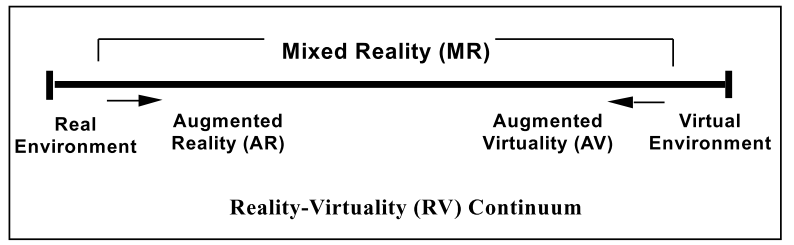
\includegraphics[width=0.8\linewidth]{images/10-intro/mixed-reality-continuum.png}
    \caption{The mixed reality continuum by Milgram \cite{Milgram1995a}}
    \label{fig:mr-continuum}
\end{figure}

We, as humans, are social creatures, and it is our way to stay connected with each other, communicating our identity and the feeling of relatedness to one another \cite{HuangWeidong2013}. Social interactions help to establish mutual understandings in collaborative scenarios and therefore, can be used as an effective measure of collaborative technology \cite{Li2013}. Social interactions have been influenced by technology. For instance, emoticons have been used in written communication instead of text to represent our emotions, intentions and cultural differences \cite{Pavalanathan2016}, and was found to be related to expressing emotions in face-to-face situations \cite{Derks2007}. 

One of the advantages of AR in communicating social dynamics is that it enables the user to interact with virtual content while keeping social connections with people around in the real world \cite{HuangWeidong2013}. Mobile AR facilitates shared spaces and experiences with remote users in a way that adds to social connections and increases user engagement. 

Having people contributing to AR content could improve the sense of community and inter-connectedness. However, when more information is shared, there is more risk of reducing the sense of privacy \cite{Olsson2013}. In a study of social interaction and mobility in AR games, \textcite{Schmalstieg_144} found that players of mobile AR games are more likely to interact with each other socially and physically, which improves the enjoyment of AR experience. AR could improve social interactions by making people more connected with each other and excited about sharing virtual experiences and making the social experience more rich with additional virtual content. 

In a review of the trends of 20 years research in AR at ISMAR\footnote{http://www.ismar.net/}, \textcite{Zhou2008, Kim2018} reported that "\textit{AR technology will continue to develop even more dynamically and effectively over the next ten years, toward the vision of pervasive presence in our daily lives.}" \cite{Kim2018}. AR displays are getting more affordable with better rendering and registration techniques. They are also becoming more self-contained and lighter, which enables mobile AR applications.

According to a review about the historical uses of wearable displays and AR displays \cite{Peddie2017}, it started in 1940 with the first heads-up display (HUD) in the UK. Then in the 1960s, most uses of AR were to build an AR helmet for the pilot's field of view. Then interest in AR started increasing in 2009 when Lego\footnote{https://www.lego.com} introduced AR Digital box, then started a relative decline around when Google Glass was introduced in 2012. The Gartner 2019 trends report \cite{gartner2019} showed that AR and immersive technologies have been getting out the "disillusionment" phase of the hype cycle and are moving toward steady adoption and day to day scenarios in the next 5-10 years.

\section{Problem Statement}

With the rapid development of technology and the potential use of AR in everyday life, this thesis aims to study the future challenges in social AR. The focus of this thesis is on enabling the use of wearable AR for sharing social experiences. The gap between the vision of social AR and the current state of the art is that state of the art in AR research has focused on task-oriented collaborative AR more than social AR. Initial attempts at exploring social AR in 2013 (at the beginning of this thesis) were limited in terms of the number of users. 
% This thesis explores how multiple people would use social AR to connect the shared virtual space and the interaction techniques. 

This PhD thesis addresses the problems of: 
\begin{enumerate}
    \item visualising and interacting with social contacts through wearable AR displays.
    \item displaying a large amount of 3D content of sharing social data that is overlaid over a limited available physical space through wearable AR devices.
    \item defining and exploring the best ways to use wearable AR devices to connect with social networks.
\end{enumerate}

Previously, hand-held AR systems have been used to view social networks in different ways. For example, Presslite's Twitter 360\footnote{https://www.youtube.com/watch?v=5w7EAz8-uwU} (Figure \ref{fig:presslite}) shows virtual tweets overlaid on the real world at the locations of the people that sent them , and early versions of Junaio\footnote{https://en.wikipedia.org/wiki/Junaio} allowed people to drop virtual messages and pictures in the real world, as did the popular application Sekai Camera\footnote{https://www.youtube.com/watch?v=oxnKOQkWwF8}. Most of these applications were focused on asynchronous collaboration, enabling people to post virtual messages in space, which can later be browsed and retrieved by other users. 

\begin{figure}
    \centering
    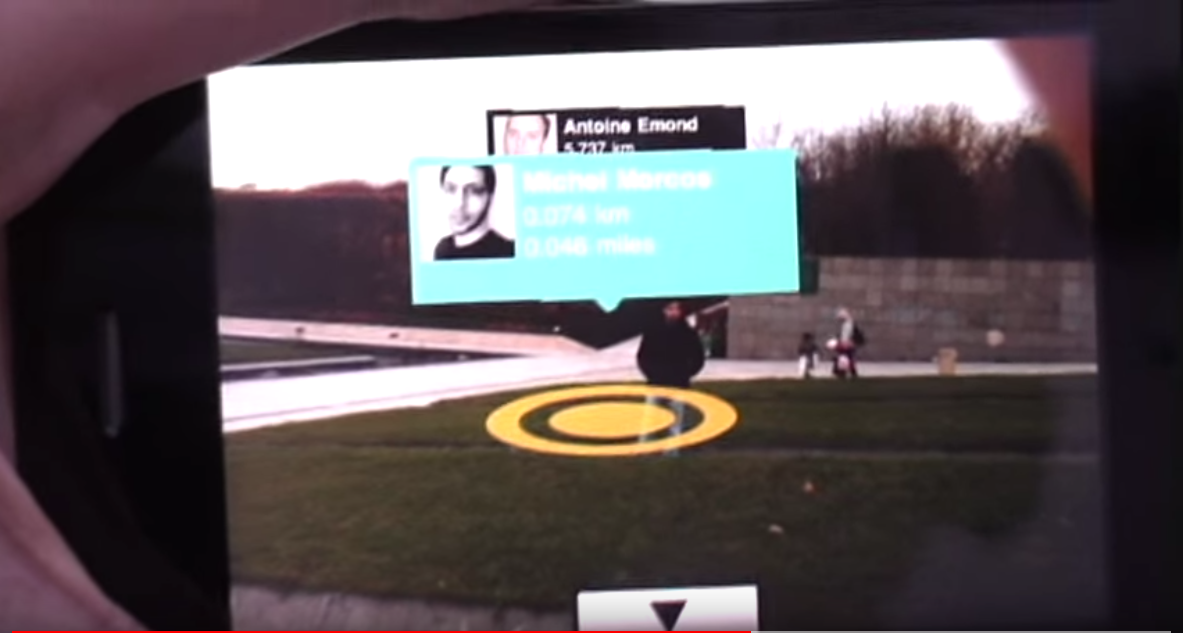
\includegraphics[width=0.8\linewidth]{images/10-intro/Presslite-twitter-360.PNG}
    \caption{Presslite's Twitter 360 AR interface by Twitter in 2009}
    \label{fig:presslite}
\end{figure}

However, similar technology could also be used for live synchronous collaboration such as live video avatar sharing~\cite{Billinghurst2002}, sharing realistic 3D models superimposed over the real world~\cite{Fanello2016}, or by using virtual avatars to show a live view of remote collaborators and their surrounding space as in the Holoportation system~\cite{Fanello2016} (Figure \ref{fig:holoportation}).

\begin{figure}
    \centering
    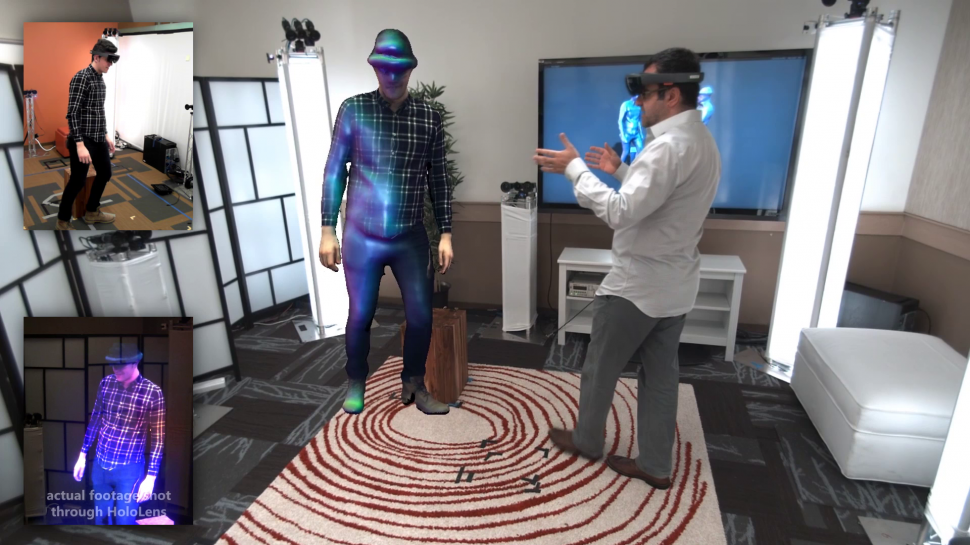
\includegraphics[width=0.8\linewidth]{images/10-intro/holoportation.png}
    \caption{Holoportation by Microsoft \cite{Fanello2016}}
    \label{fig:holoportation}
\end{figure}

% - The potential for AR to be a social sharing platform. \\
% - Sharing social experiences was not fully addressed in the research community

With major industry players (e.g., Microsoft, Facebook and Magic Leap) building solutions in AR, there is potential for use of AR in social networks. Just as people today use their mobile phones to connect with hundreds or thousands of friends, wearable AR displays could be used to connect with friends and view and interact with their shared information.

Applications for Social VR and 360-degree video have been introduced on new VR headsets. For instance, Facebook Spaces\footnote{https://www.facebook.com/spaces} allows VR users to connect with friends and family and share 360-degree photos and take selfies. Altspace VR\footnote{https://altvr.com/} is a social VR application which was acquired by Microsoft and has been extended to support different hand-held and wearable devices to be used for social connection with others. Most recently, Magic Leap's Avatar Chat\footnote{https://www.magicleap.com/stories/blog/connect-with-friends-with-avatar-chat}(Figure \ref{fig:ml-avatar-chat-1}) offers similar experiences where avatars representing social friends are displayed in an AR space. 

\begin{figure}
    \centering
    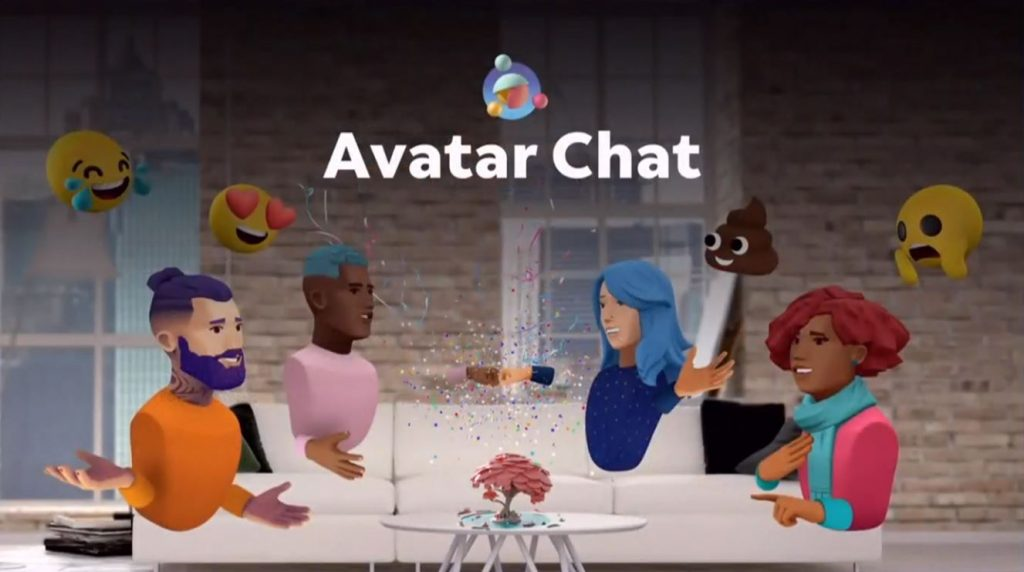
\includegraphics[width=0.8\linewidth]{images/10-intro/magic-leap-avatar-chat.jpg}
    \caption{Avatar Chat by Magic Leap, 2018}
    \label{fig:ml-avatar-chat-1}
\end{figure}

By using a wearable AR display like the Microsoft HoloLens\footnote{https://www.microsoft.com/en-nz/hololens}, it could be possible for the user to see an AR representation of their social network visible at all times. However, this raises the question of how to visually represent the user's contacts in the network. For example, if a user has lots of friends in their social network, visually representing each of them might clutter the user's visual space.

The limitation of prior work is that until recently (2018), there was no comprehensive analysis of the social AR space and no sufficient exploration of sharing social experiences on wearable AR. It is easy to imagine that in the future it will be possible for wearable AR systems to be used to capture and share a 3D view of the user's surroundings with hundreds or thousands of followers on a social network. However, before this becomes commonplace, many important research questions need to be addressed. For example, would a person be comfortable sharing a view of their surrounding real space with relative strangers? This work aims to explore how wearable AR systems could share a user's surrounding room environment with social contacts and to measure how comfortable the sharer and the viewer would feel regarding privacy within different interface options. 

If AR is to be used to represent contacts in social networks, there could be a large number of contacts to show. This research has benefited from earlier work on different ways of managing large amounts of information in AR interfaces. In the following section, this thesis outlines the research questions based on the above problem space and the gap identified in previous work.

\section{Research Questions}

This thesis targets the future where headworm AR devices are used every day, and social networks are visualised in the AR view. The overarching research question is \textit{how can AR be used for sharing social experiences in both remote and face to face social contacts}. This thesis addresses the following research questions: 

\begin{enumerate}[label=RQ\arabic*]
    % (chapter 3 - Social AR Continuum)
    \item{\label{rq:continuum}
    What are the dimensions/factors/parameters in sharing social experiences on wearable AR devices?
    % \\(option 1): How to represent social networks and shared social data on wearable AR devices?
    % \\(option 2): What dimensions/factors/parameters in sharing social experiences on wearable AR devices?
    }
    % (chapter 4 - visualising social contacts) 
    \item{\label{rq:people}
    What dimensions work best for visualising and interacting with social contacts through wearable AR displays?
    % \\(option 1): How to visualise our social contacts as virtual avatars on wearable AR devices?
    % \\(option 2): What are the options of visualising contacts on social AR?
    % \\(option 3): How visualising social contacts are placed on the Social AR Continuum?
    % \\(option 4): What is the impact of visualising social contacts on social presence?
    % \\(option 5): What is the impact on social presence of different visualisation methods for social contacts?
    }
    % (chapter 5 - Social data continuum)
    \item{\label{rq:data}
    How does social proximity affect visualising and interaction with shared social data on wearable AR displays?
    % What dimensions are best to visualise and interact with shared social data on wearable AR displays?
    % What is the best way to view and interact with shared social data on AR displays?
    % \\(option 1): How to share virtual objects/data with our social network on wearable AR devices?
    % \\(option 2): What are the options of sharing social data in AR?
    % \\(option 3): How sharing data is placed on the Social AR Continuum?
    }
    % (chapter 4 - social interaction continuum)
    \item{\label{rq:interaction}
    How can wearable AR displays be used best for interacting with social contacts and shared social data?
    % \\(option 1): How to represent annotations/tags on wearable AR devices for shared social experiences?
    % \\(option 2): How annotations/tags are used as an interaction method in social AR? 
    % \\(option 3): What are the options/parameters of annotation that can be changed in social AR?
    }
\end{enumerate}

In order to answer the research questions, this thesis explores how wearable AR can be used for sharing social experiences. These explorations identified the parameters through which AR sharing for social reasons happens. Once the parameters were defined, system prototypes were built as a proof of concept of how users can experience those dimensions. User studies were approved by the Human Ethics Committee (HEC) and aimed to test the objectives of each system with human participants. Outcomes of user studies include subjective and objective measures and observations of users' behaviour and feedback from going through these experiments. 

Chapter \ref{ch:continuum}: "The Social AR Continuum" aims to answer \ref{rq:continuum} with describing the overall dimensions of the Social AR Continuum. 
Chapter \ref{ch:contacts} "Visualising Social Contacts" aims to answer \ref{rq:people} by exploring visualising social contacts. 
Chapter \ref{ch:data} "Sharing Data Continuum" focuses more on the data being shared with social contacts and aiming to answer \ref{rq:data}.
Chapter \ref{ch:annotation} "Annotation Continuum" aims to answer \ref{rq:interaction} with exploring annotations and tags for sharing social experience. 

\section{Contributions}

The following summarises the contributions of this thesis: 

\begin{itemize}
    \item The parameters and dimensions of the Social AR Continuum were identified. The main contribution is defining the Social AR Continuum, which consists of a set of parameters that define the space of sharing social experiences through wearable/hand-held AR devices. Following the identification, this thesis defines the space of the Social AR Continuum by exploring the main parameters that can be varied based on social proximity. These parameters are grouped into the following categories 1) self and other, 2) shared objects \& surrounding environment and 3) interactions and annotations. Under each of these categories, this thesis defines the dimensions of variables that affect the shared social experience.
    
    \item Several social AR experiences in terms of user interfaces were implemented. For each dimension defined on the continuum, a system prototype was built to test the user interface design with human subjects. The implementation details are described in the thesis for future use.
    
    \item User studies were conducted to evaluate and validate the parameters of the Social AR Continuum. The prototypes then used in a series of user-studies and focus-groups were conducted to validate the dimensions of the Social AR Continuum.
    
    \item High-level design guidelines were synthesised for interface designers looking to build social sharing experiences on AR devices. One of the outcomes of defining the Social AR Continuum and validating these dimensions is that this work can serve as high-level experience design guidelines that help individuals and organisations to create effective AR experiences for social sharing and connection purposes.
\end{itemize}

In summary, this thesis helps to increase the understanding of how to share social experiences through AR devices. The results of the user experiments conducted throughout this research help identify the impact of the Social AR Continuum parameters on presence, user engagement and user interface usability, which serve as guidelines for future designs. 

Figure \ref{fig:thesis-outline} shows the structure of the thesis and how it answers the research questions. The thesis is organised as follows: Chapter \ref{ch:continuum} describes the Social AR Continuum and the parameters/dimensions involved. 
Chapter \ref{ch:contacts} focuses on the dimensions of self and others of representing social contact networks on AR devices. 
Chapter \ref{ch:data} studies the shared social data and surrounding environment dimensions, including shared 360-degree videos and 3D captured spaces. 
In chapter \ref{ch:annotation}, this thesis looks into the shared data and annotation continuum, including different implementations of shared annotation and awareness cues on different platforms (hand-held and wearable).


\begin{figure}
    \centering
    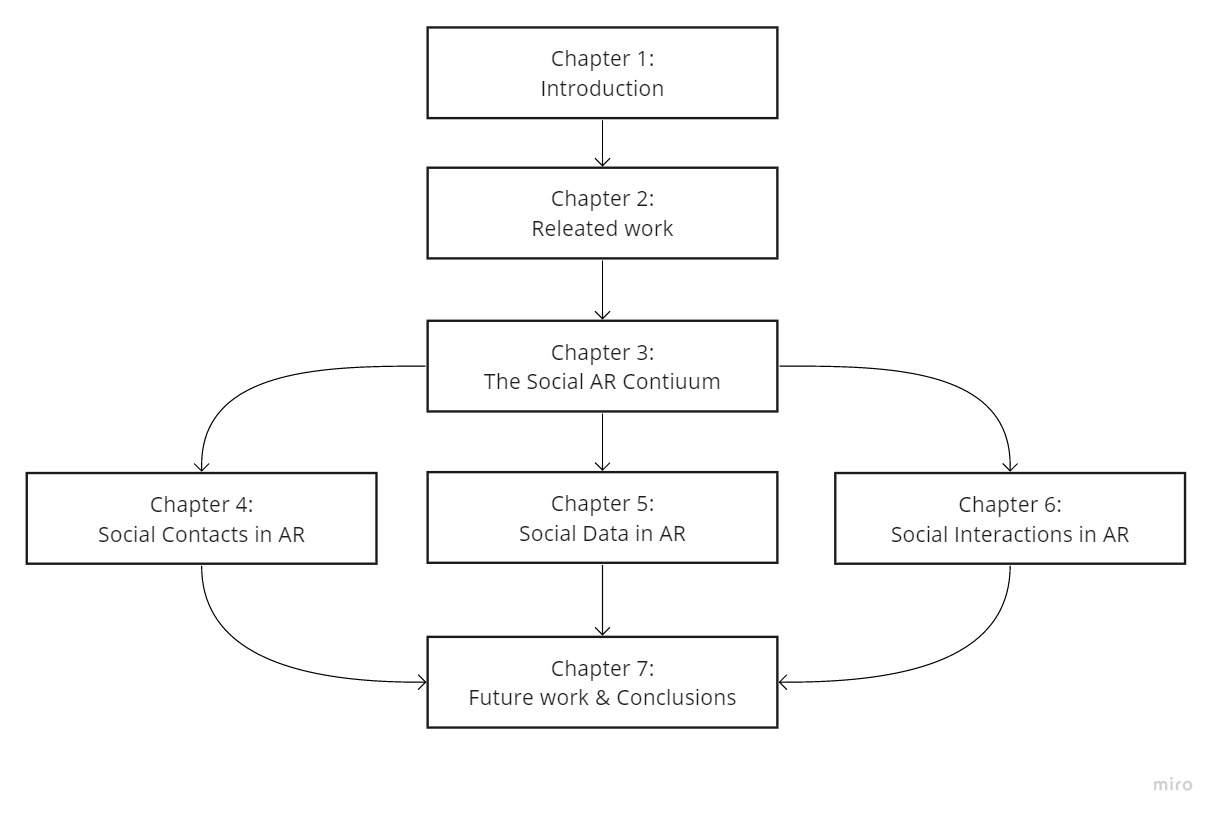
\includegraphics[width=\linewidth]{images/10-intro/thesis-outline.jpg}
    \caption{Thesis outline}
    \label{fig:thesis-outline}
\end{figure}

\section{Selected Publications}
\preto\fullcite{\AtNextCite{\defcounter{maxnames}{99}}}

Most of the work in this thesis has been submitted, peer-reviewed and published at scientific conferences and journals specialising in the AR, HCI and computer graphics fields. This list contains selected publications that are relevant to this thesis. 

The following publication defines the concept of the Social AR Continuum and describes a focus group and a user study implementing visualising social contacts through an AR headset, and addressing \ref{rq:continuum}. 

\begin{itemize}
    \item{ \fullcite{Nassani2017a}}
\end{itemize}

The following publications focus on visualising social contacts based on social proximity, addressing \ref{rq:people}. 

\begin{itemize}
    \item{ \fullcite{Nassani2017b}}
    \item{ \fullcite{Nassani2017}}
\end{itemize}

The following publications focus on shared surrounding environments and changing the levels of detail based on social proximity, addressing \ref{rq:data}.

\begin{itemize}
    \item{ \fullcite{Nassani2018a}}
    \item{ \fullcite{Nassani2018b}}
    % \item{ \fullcite{Nassani2018c}} -- frontier paper rejected
\end{itemize}


The following publications focus on placing AR annotations/tags on shared 360-degree panoramas and video streaming content, addressing \ref{rq:interaction}.

\begin{itemize}
    \item{ \fullcite{Nassani2016}}
    \item{ \fullcite{Nassani2015}}
    % \item{ \fullcite{Nassani2015a}}    
    \item{ \fullcite{Reichherzer2014}}
    % \item{ \fullcite{Billinghurst2014}}
\end{itemize}
The above publications help to answer the research questions of this thesis, including how to share social experiences on AR devices for each category on the Social AR Continuum. 
